\documentclass[a4paper,12pt]{article}
%Inclucdnutie packagov
\usepackage[slovak]{babel}
\usepackage[utf8]{inputenc}
\usepackage{amsmath}
\usepackage[bookmarksopen,colorlinks,plainpages=false,urlcolor=blue]{hyperref}


\usepackage{url}

\usepackage{ifpdf}

% \ifthenelse{\isundefined{\pdfoutput}}
\ifpdf
  \usepackage[dvipdf]{graphicx}
\else
  \usepackage[dvips]{graphicx}
\fi

\usepackage[top=2cm, left=2cm, text={17cm, 26cm}, ignorefoot]{geometry}
\author{Dávid Mikuš - xmikus15}
\title{ITO}
%Zaciatok dokumentu
\begin{document}

\begin{figure}[!h]
  \centering
  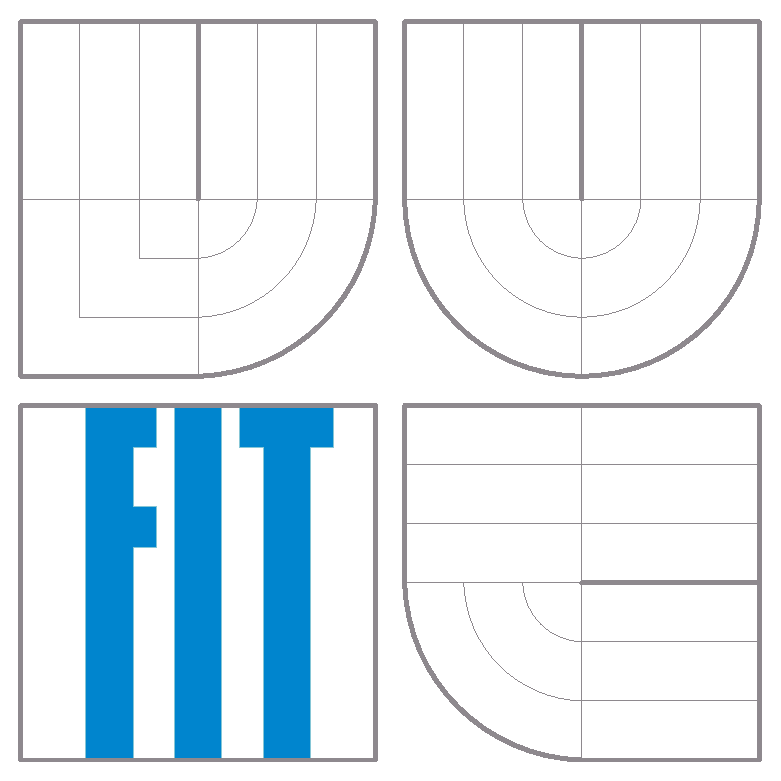
\includegraphics[height=5cm]{img/logo}
\end{figure}

\begin{center}
\bigskip
\begin{Huge}
Teória obvodov 2013/2014\\
\end{Huge}
\begin{large}
Projekt
\end{large}
\end{center}

\begin{center}
\begin{Large}
\today
\end{Large}
\end{center}

\vfill

\begin{flushleft}
\begin{large}
\begin{tabular}{ll}
Autor: & Dávid Mikuš, \url{xmikus15@stud.fit.vutbr.cz} \\
 & Fakulta Informačních Technologií \\
 & Vysoké Učení Technické v~Brně \\
\end{tabular}
\end{large}
\end{flushleft}

% % % % % % % % % % % % % % % % % % % % % % % % % % % % % % % % % % % % % % % % % % % % % % % %
\newpage
\begin{center}
\textbf{Priklad 1, Varianta F}
\end{center}
\bigskip
Stanovte napätie 
\textcolor{red}{$U_{R7}$}
a prúd
\textcolor{red}{$I_{R7}$}.
Použite metódu postupńeho zjednosušovania obvodu.
\bigskip

Zadané hodnoty

\begin{tabular} {|  c | c | c | c | c | c | c | c | c | }
\hline
U[V] & $R_1[\Omega]$ & $R_2[\Omega]$ & $R_3[\Omega]$ & $R_4[\Omega]$ & $R_5[\Omega]$ & $R_6[\Omega]$ & $R_7[\Omega]$ & $R_8[\Omega]$\\ \hline
125 & 510 & 500 & 550 & 250 & 300 & 800 & 330 & 250 \\ \hline
\end{tabular}
\bigskip

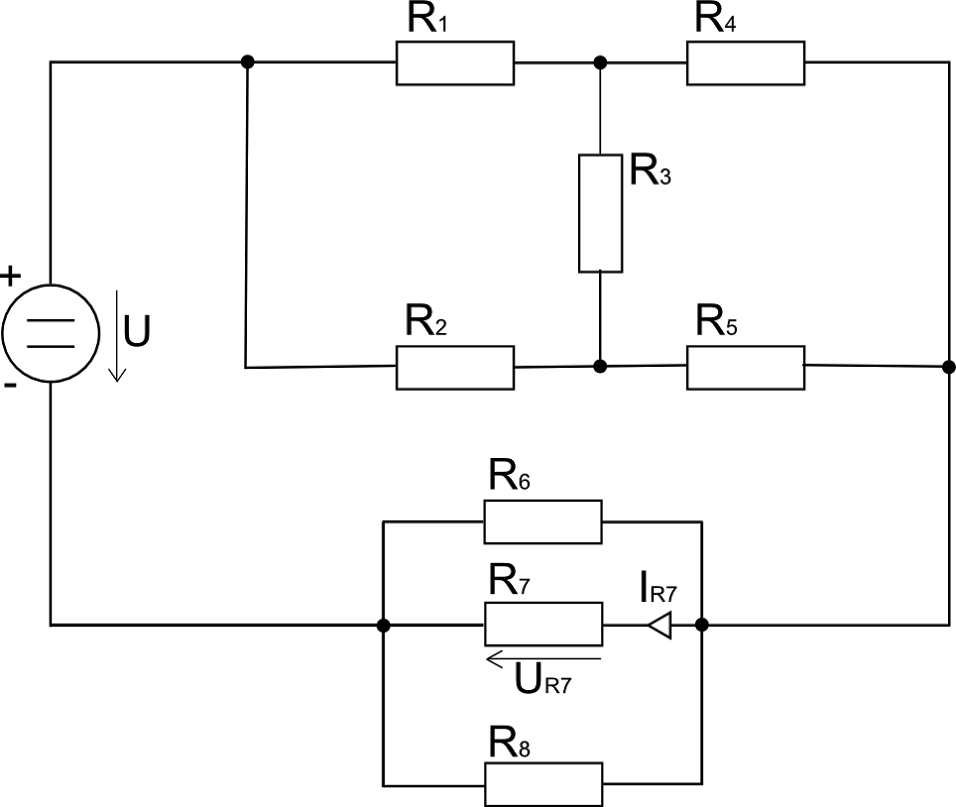
\includegraphics[height=10cm]{img/pr1a}

\bigskip
1. Obvod transfigurujeme na hviezdu

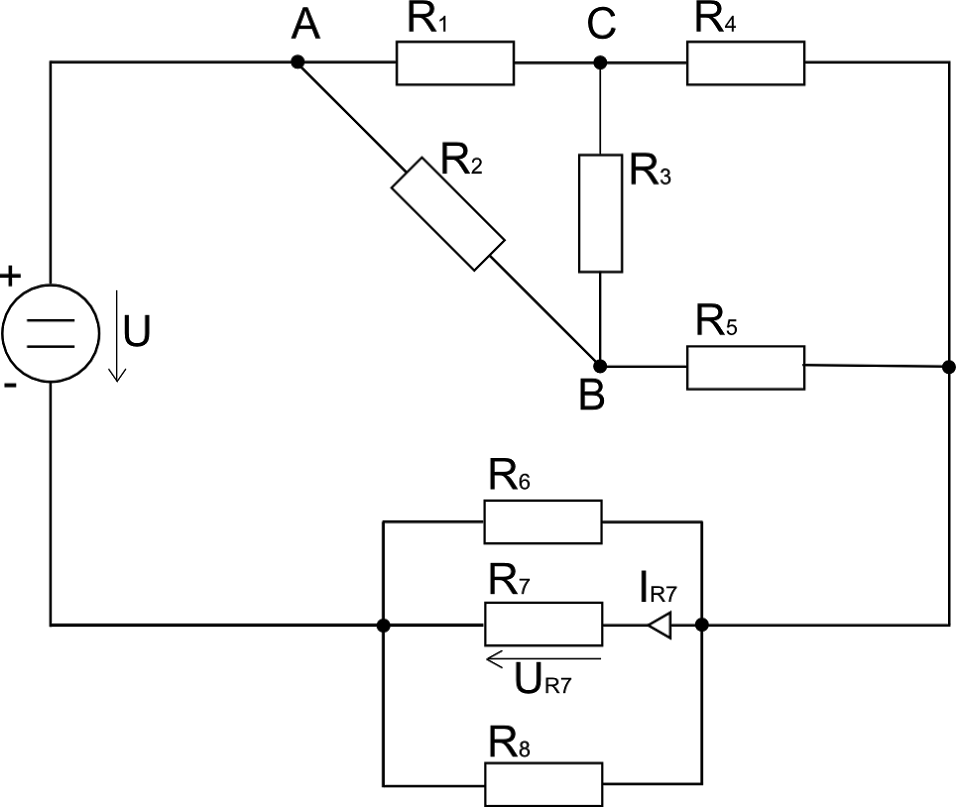
\includegraphics[height=6cm]{img/pr1b}
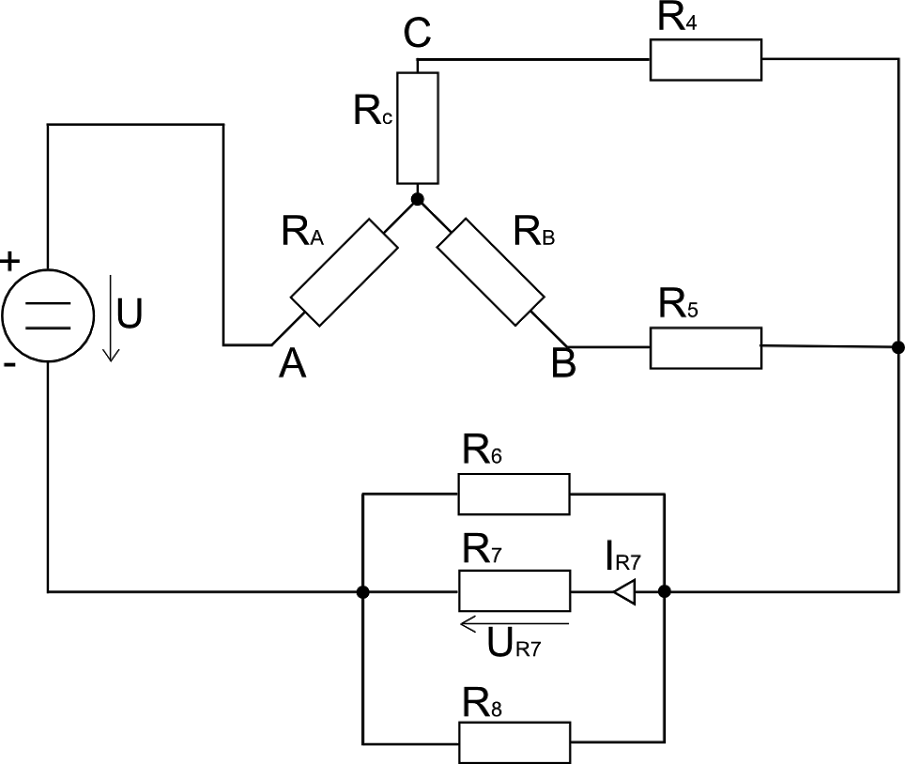
\includegraphics[height=6cm]{img/pr1c}

\bigskip
\begin{equation*}
R_A = \frac{R_1 * R_2}{ R_1 + R_2 + R_3} = \frac{510\Omega*500\Omega}{510\Omega+500\Omega+550\Omega} = 163,4615\Omega
\end{equation*}
\begin{equation*}
R_B = \frac{R_2 * R_3}{ R_1 + R_2 + R_3} = \frac{500\Omega*550\Omega}{510\Omega+500\Omega+550\Omega} = 176,2820\Omega
\end{equation*}
\begin{equation*}
R_C = \frac{R_1 * R_3}{ R_1 + R_2 + R_3} = \frac{510\Omega*550\Omega}{510\Omega+500\Omega+550\Omega} = 179,8076\Omega
\end{equation*}

\newpage

2 .$R_C$ a $R_4$ sú sériovo zapojené, zjednotíme ich. Tak isto aj $R_B$ a $R_5$

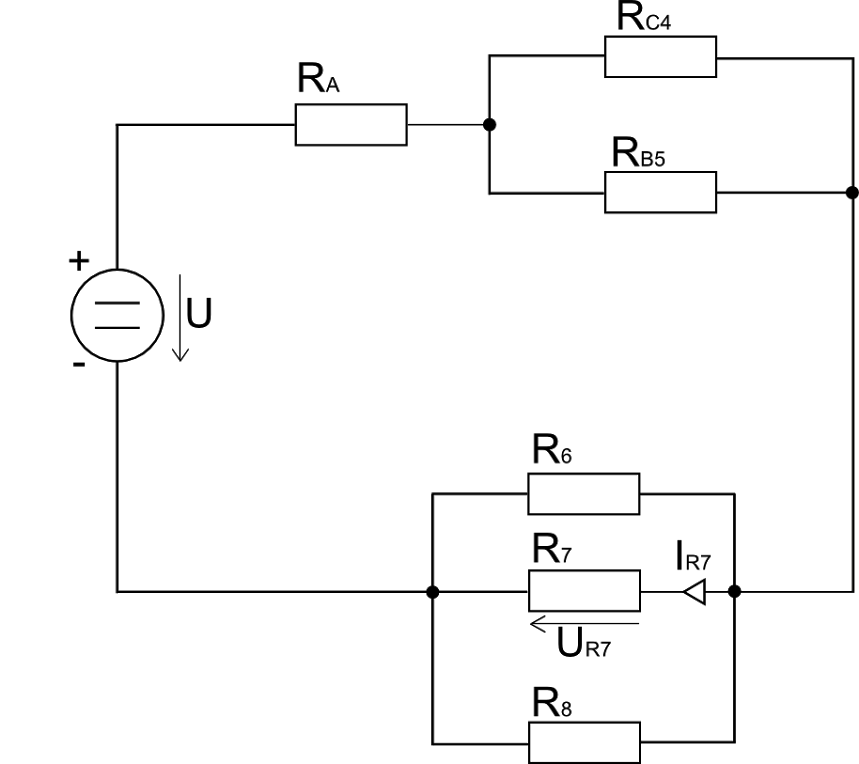
\includegraphics[height=6cm]{img/pr1d}

\begin{equation*}
R_{C4} = R_C + R_4 = 179,8076\Omega + 250\Omega = 429,8076\Omega
\end{equation*}
\begin{equation*}
R_{B5} = R_B + R_5 = 176,2820\Omega + 300\Omega = 476,2821\Omega
\end{equation*}

3. $R_{C4}$ a $R_{B5}$ sú parelne zapojené. Spočítame ich.

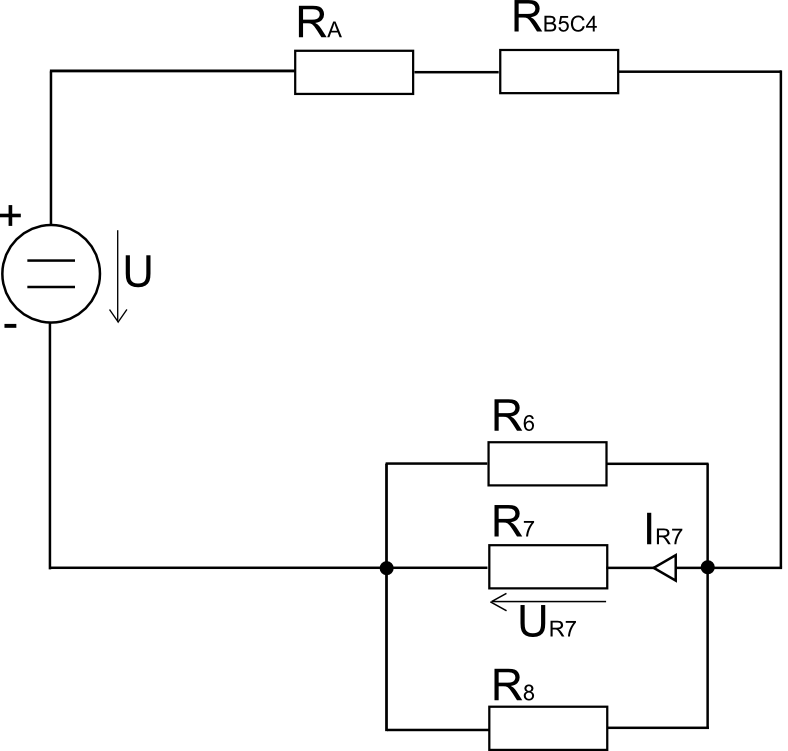
\includegraphics[height=6cm]{img/pr1e}

\begin{equation*}
R_{B5C4} = \frac{R_{C4} *  R_{B5}}{R_{C4} + R_{B5}}  = \frac{429,8076\Omega * 476,2821\Omega}{429,8076\Omega + 476,2821\Omega} = 225,9265\Omega
\end{equation*}


4. $R_6$ , $R_7$ a $R_8$ sú parelne zapojené.

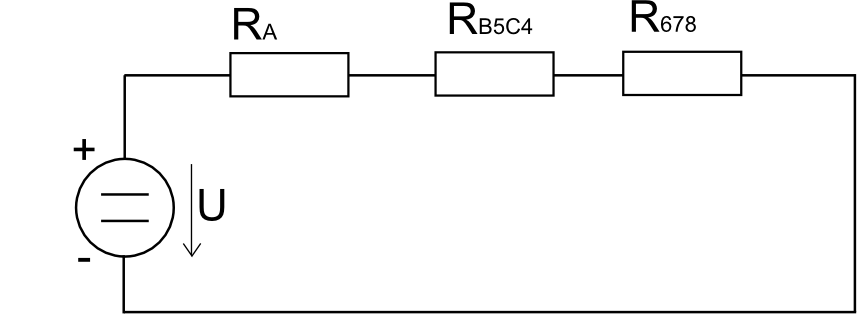
\includegraphics[height=5cm]{img/pr1f}

\begin{equation*}
R_{678} = \frac{R_6*R_7*R_8}{R_6*R_7+R_6*R_8+R_7*R_8} = \frac{800\Omega*330\Omega*250\Omega}{800\Omega*330\Omega+800\Omega*250\Omega+330\Omega*250\Omega} = 120,7685\Omega
\end{equation*}
\newpage

5. Vypočítame celkový odpor obvodu.

\begin{equation*}
R = R_A + R_{B5C4} + R_{678} = 163,4615\Omega + 225,9265\Omega + 120,7685\Omega =  510,1566\Omega
\end{equation*}


6. Pomocou ohmovho zákona vypočítame celkový prúd.
\begin{equation*}
I=\frac{U}{R} = \frac{125V}{510,1566\Omega} = 0.2450A
\end{equation*}

7. Spočítame odpor $R_{AB5C4}$, čo je celkový odpor prúd okrem $R_{678}$

\begin{equation*}
R_{AB5C4} = R - R_{678} = 510,1566\Omega - 120,7685\Omega = 389,3880\Omega
\end{equation*}

 8. Vypočítame napätie $U_{AB5C4}$ a následne môžme určiť $U_{678}$

\begin{equation*}
U_{AB5C4} = R_{AB5C4} * I = 389,3880\Omega * 0.2450A = 95,4089V
\end{equation*}

\begin{equation*}
U_{678} = U - U{AB5C4} = 125V - 95,4089V = 29,6001V
\end{equation*}

9. Nakoniec určime \textcolor{red}{$U_{R7}$} a \textcolor{red}{$I_{R7}$}. . Prúd $I_{678}$ je rovný celkovému prúdu na obovde. 

\begin{equation*}
 I_{678} = I = 0,2450 A
\end{equation*}

\begin{equation*}
U_{R7} = U_{678} = 29,6001 V
\end{equation*}

\begin{equation*}
I_{R7} = \frac{U_{678}}{R_7} = \frac{29,6001V}{330\Omega} = 0,0896A
\end{equation*}

\newpage

% % % % % % % % % %  2. Priklad % % % % % % % % % % % % % % % % % % % % % % % % 
\begin{center}
\textbf{Priklad 2, Varianta H}
\end{center}
\bigskip
Stanovte napätie 
\textcolor{red}{$U_{R5}$}
a prúd
\textcolor{red}{$I_{R5}$}.
Použite metódu Theveninovej vety.
\bigskip

Zadané hodnoty

\begin{tabular} {|  c | c |  c | c | c | c | }
\hline
U[V] & $R_1[\Omega]$ & $R_2[\Omega]$ & $R_3[\Omega]$ & $R_4[\Omega]$ & $R_5[\Omega]$\\ \hline
220 & 360 & 580 & 205 & 360 & 350 \\ \hline
\end{tabular}
\bigskip

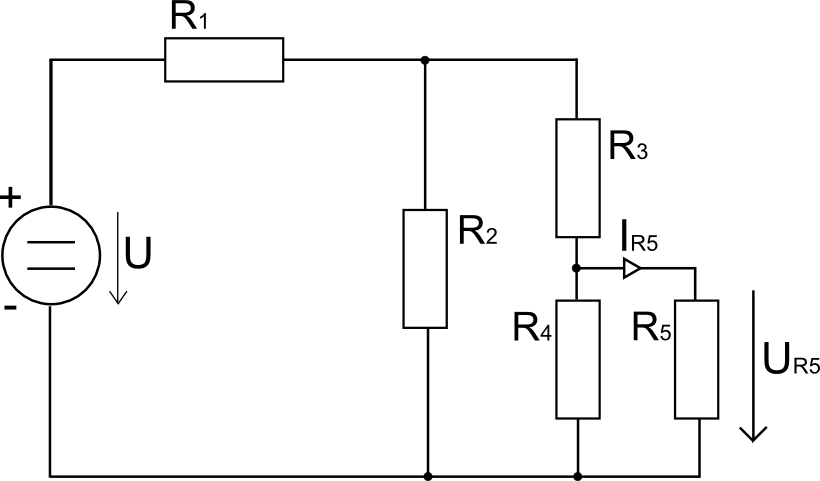
\includegraphics[height=5cm]{img/pr2a}

1. Vyskratujeme $R_5$ a zjednodušíme:

\begin{equation*}
R_{34} = R_3 + R_4= 205\Omega + 360\Omega = 565\Omega
\end{equation*}

\begin{equation*}
R_{234} = \frac{R_2*R_{34}}{R_2+R_{34}} = \frac{580\Omega*565\Omega}{580\Omega + 565\Omega} = 286,2009\Omega
\end{equation*}

\begin{equation*}
R_{1234}= R_1 + R_{234} = 360\Omega + 286,2009\Omega =  646,2009\Omega
\end{equation*}

2. Dopočítame napätia a prúdy

\begin{equation*}
I_1 = \frac{U}{R_{1234}} = \frac{220V}{646,2009\Omega} = 0,3405A
\end{equation*}

\begin{equation*}
U_{R1} = I_1 * R_1 =  0,3405 A * 360\Omega = 122,5625V
\end{equation*}

\begin{equation*}
U_{R2} =U - U{R1} = 220V - 122,5625V = 97,4375V
\end{equation*}

\begin{equation*}
I_2 = \frac{U{R2}}{R_2} = \frac{97,4375V}{580\Omega} = 0,1680A
\end{equation*}

\begin{equation*}
I_3 = I_1 - I_2 =  0,3405A - 0,1680A = 0,1725A
\end{equation*}

3. Náhradny obvod podla theveninovej vety vyzerá tsakto: 

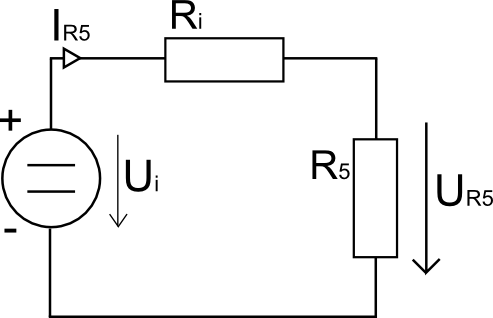
\includegraphics[height=5cm]{img/pr2b}

4. Vypočitame $R_i$ a $U_i$

\begin{equation*}
U_i = R_4 * I_3 = 360\Omega * 0,1725A = 62,0841V
\end{equation*}

\begin{equation*}
R_i = \frac{(\frac{R_1 * R_2}{R_1+R_2} + R_3) * R_4} {(\frac{R_1 * R_2}{R_1+R_2} + R_3)+R_4} = \frac{(\frac{360\Omega * 580\Omega}{360\Omega+580\Omega} + 205\Omega) * 360\Omega} {(\frac{360\Omega* 580\Omega}{360\Omega+580\Omega} + 205\Omega)+360\Omega} = 195,3507\Omega
\end{equation*}

5. Vypočítame výsledny \textcolor{red}{$U_{R5}$} a \textcolor{red}{$I_{R5}$}.

\begin{equation*}
I_{R5} = \frac{U_i}{R_i+R_5} = \frac{62,0841V}{195,3507\Omega + 350\Omega} = 0,1138A
\end{equation*}

\begin{equation*}
U_{R5} = I_{R5} * R_5 =  0,1138 A * 350\Omega = 39,8449V
\end{equation*}

% % % % % % % % % %  3. Priklad % % % % % % % % % % % % % % % % % % % % % % % % 
\newpage
\begin{center}
\textbf{Priklad 3, Varianta D}
\end{center}
\bigskip
Stanovte napätie 
\textcolor{red}{$U_{R4}$}
a prúd
\textcolor{red}{$I_{R4}$}.
Použite metódu uzlových napätí ($U_A$, $U_B$,  $U_C$). 
\bigskip

Zadané hodnoty

\begin{tabular} {|  c | c |  c | c | c | c | c | c | }
\hline
U[V]  & $I_1 [A]$ & $I_2[A]$ & $R_1 [\Omega]$  & $R_2 [\Omega]$  &$R_3 [\Omega]$  &$R_4[\Omega]$  & $R_5[\Omega]$ \\ \hline
115 & 60 & 0.9 & 500 & 380 & 480 & 370 & 285\\ \hline
\end{tabular}
\bigskip

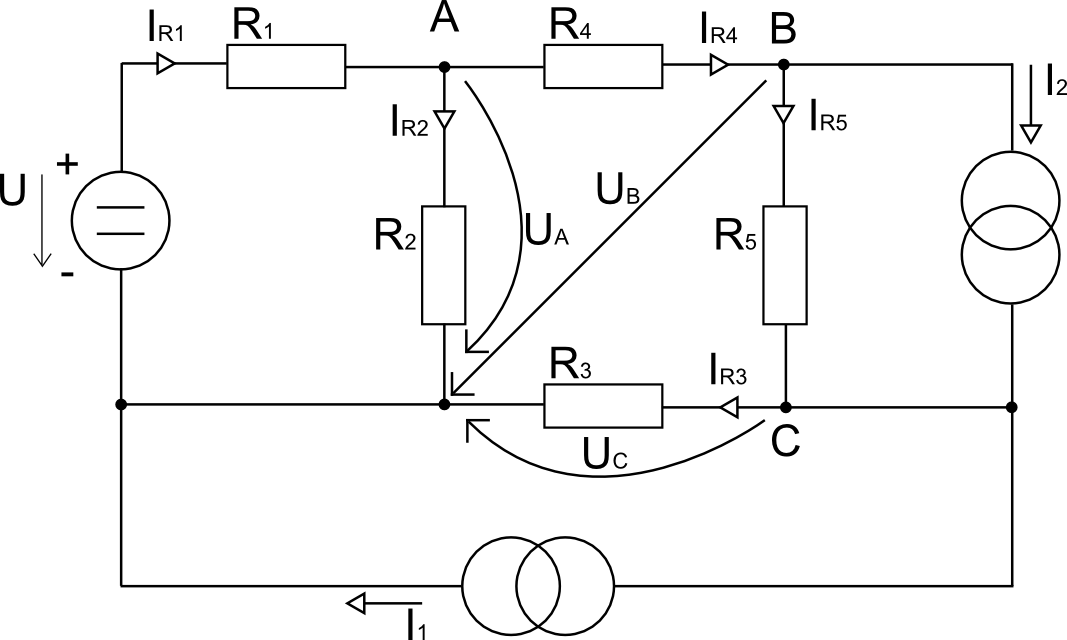
\includegraphics[height=6cm]{img/pr3a}

1. Pre každý uzol vytvoríme rovnice, podľa ktorých dopočítame $U_A$, $U_B$, $U_C$
\begin{equation*}
A: I_{R1} - I_{R2} - I_{R4} = 0
\end{equation*}
\begin{equation*}
B: I_{R4} - I_{R5} - I_2 = 0
\end{equation*}
\begin{equation*}
C: I_{R5} + I_2 - I_{R3} = 0
\end{equation*}

2. Pomocou 2. Kirchhoffova zákona zostavíme rovnice pre prúdy.

\begin{equation*}
\begin{split}
R_1 * I_{R1} + U_A - U &= 0 => I_{R1} = \frac{U-U_A}{R_1} \\
R_2 * I_{R2} - U_A&= 0 =>I_{R2} = \frac{U_A}{R_2} \\
R_3 * I_{R3} - U_C &=0 => I_{R3} = \frac{U_C}{R_3} \\
R_4 * I_{R4}+ U_B- U_A &= 0 => I_{R4} = \frac{U_A-U_B}{R_4} \\
R_5 * I_{R5} + U_C - U_B &= 0 => I_{R5} = \frac{U_B-U_C}{R_5}
\end{split}
\end{equation*}

3. Rovnce dosadime
\begin{equation*}
    \begin{split}
	A: \frac{U-U_a}{R_1} - \frac{U_A}{R_2} - \frac{U_A-U_B}{R_4} = 0 \\
	B: \frac{U_A-U_B}{R_4} - \frac{U_B - U_C}{R_5} - I_2 = 0 \\
	C: \frac{U_B-U_C}{R_5} + I_2 - I_1 - \frac{U_C}{R_3} = 0
    \end{split}
\end{equation*}
\hrulefill

\begin{equation*}
    \begin{split}
	R_2 * R_4 * U - R_2 * R_4 * U_A - R_1 * R_4 * U_A - R_1 * R_2 * U_A + R_1 * R_2 * U_B = 0 \\
	R_5 * U_A - R_5 * U_B - R_4 * U_B + R_4 * U_C - R_4 * R_5 * I_2 = 0 \\
	R_3 * U_B - R_3 * U_C + R_3 * R_5 * I_2 -R_3*R_5*I_1 -R_5*U_C = 0
    \end{split}
\end{equation*}
\hrulefill

\begin{equation*}
    \begin{split}
	-U_A * (R_1*R_2+R_2*R_4 +R_1 * R_4) + U_B *R_1 *R_2 &= -U*R_2* R_4 \\
	U_A * R_5 - U_B * (R_4+R_5) + U_C * R_4 &= R_4 * R_5 * I_2 \\
	U_B * R_3 - U_C * (R_3+R_5)&= R_3* R_5*(I_1-I_2)
    \end{split}
\end{equation*}
\hrulefill

\begin{equation*}
    \begin{split}
	-U_A * (500\Omega*380\Omega+380\Omega*370\Omega +500\Omega * 370\Omega) + U_B *500\Omega *380\Omega &= -115V *380\Omega* 370\Omega \\
	U_A * 285\Omega - U_B * (370\Omega+285\Omega) + U_C * 370\Omega &= 370\Omega * 285\Omega * 0.9A \\
	U_B * 480\Omega - U_C * (480\Omega+285\Omega)&= 480\Omega* 285\Omega*(60A-0.9A)
    \end{split}
\end{equation*}

3. Dostávame maticu:
\begin{equation*}
M = \begin{bmatrix}
	-2578 & 950 & 0 & -80845 \\
	57 & -131 & 74 & 18 981 \\
	0 & 32 & -51 & 538992
     \end{bmatrix}
\end{equation*}

4. Vypočítame $U_A$ a $U_B$ pomocou determinantov.
\begin{equation*}
M_0 = \begin{bmatrix}
	-2578 & 950 & 0  \\
	57 & -131 & 74  \\
	0 & 32 & -51 \\
     \end{bmatrix}
M_1 = \begin{bmatrix}
	-80845  & 950 & 0  \\
	18 981 & -131 & 74  \\
	538992 & 32 & -51 \\
     \end{bmatrix}
M_2 = \begin{bmatrix}
	-2578 &  -80845 & 0  \\
	57 & -18 981 & 74  \\
	0 & 538992 & -51 \\
     \end{bmatrix}
\end{equation*}
\begin{equation*}
   \begin{split}
	det(M_0) &= -2578 * (-131) * (-51) - (-2578*32*74) - 950*57*(-51) = - 8 357 264 \\
	det(M_1) &= -80 845 *(-131) * (-51) + 950 *74 * 538 992 - (-80 845) * 74 * 32 - 950 * 18981 * (-51) = \\
	&= 38 462 082 565 \\
	det(M_2) &= -2578 * 18981 * (-51) - (-2578) * 74 * 538992 - (-80845) * 57 * (-51) =  \\
	&= 105085149327 \\
	U_A &= \frac{det(M_1)}{det(M_0)}= \frac{38 462 082 565}{ - 8 357 264}= -4602,2340V \\
	U_B &= \frac{det(M_2)}{det(M_0)}= \frac{105085149327}{ - 8 357 264}=   -12574,1090V 
   \end{split}
\end{equation*}

5. Následne už len vypočítame  napätie 
\textcolor{red}{$U_{R4}$}
a prúd
\textcolor{red}{$I_{R4}$}.

\begin{equation*}
   \begin{split}
	U_{R4} = U_A - U_B = -4602,2340V  - (-12574,1090V ) = 7 967,875V \\
	I_{R4} = \frac{U_A-U_B}{R_4} = \frac{-4602,2340V  - (-12574,1090V )}{370\Omega} = 21,5348A
   \end{split}
\end{equation*}

% % % % % % % % % %  4. Priklad % % % % % % % % % % % % % % % % % % % % % % % % 
\newpage
\begin{center}
\textbf{Priklad 4, Varianta F}
\end{center}
\bigskip
Pre napájacie napätie platí: $\mu = U * \sin (2\pi\omega ft)$. Vo vzťahu pre napätie na kondenzátore $C_1: \mu_{C_1} = U_{C_1} * \sin (2\pi ft + \varphi_{C_1})$ určite $|U_{C_1}| a \varphi_{C_1}$.
Použite metódu zjednosušovania obvodu.

Pozn: Pomocný "smer šípky napájacieho zdroja platí pre špecialny časový okamžik $(t = \frac{\pi}{2\omega})$.""
\bigskip

Zadané hodnoty

\begin{tabular} {|  c | c |  c | c | c | c | c | c | c | }
\hline
U[V] &  $R_1 [\Omega]$  & $R_2 [\Omega]$  &$R_3 [\Omega]$  & $L_1 [mH]$ & $L_2 [mH]$ & $C_1[\mu F]$ & $C_2[\mu F]$  & f [Hz] \\ \hline
75 & 165 & 150 & 380 & 430 & 320 & 310 & 235 & 95\\ \hline
\end{tabular}
\bigskip

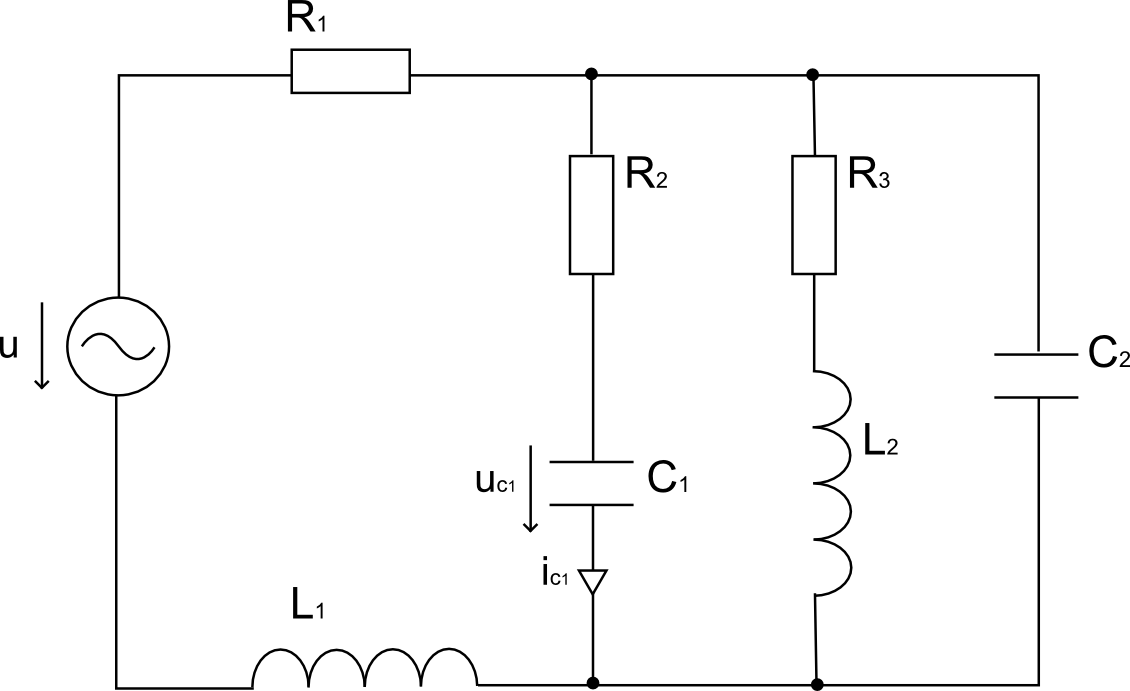
\includegraphics[height=6cm]{img/pr4a}

1. Obvod prekreslíme tak aby sa v ňom vyskytovali iba rezistory, ktoré budú reprezentovať impedancie jednotlivých vetví.

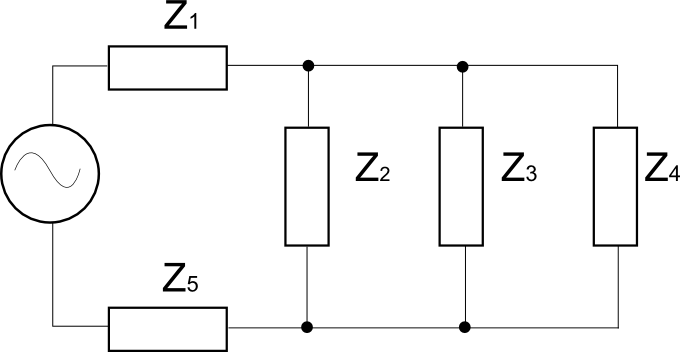
\includegraphics[height=6cm]{img/pr4b} \\
	$Z_1$ - impedancia rezistoru $R_1$  \\
	$Z_2$ - impedancia rezistoru $R_2$ a kondenzátora $C_1$ \\
	$Z_3$ - impedancia rezistoru $R_3$ a cievky $L_2$  \\
	$Z_4$ - impedancia kondenzátora $C_2$  \\
	$Z_5$ - impedancia cievky $L_1$  \\

2. Vypočítame uhlovú rýchlosť
\begin {equation*}
	\omega = 2\pi f = 2\pi * 95Hz = 596,9026 rad/s
\end {equation*}
\newpage
3. Vypočítame impedancie
\begin {equation*}
    \begin{split}
	Z_1 &= R_1 = 165\Omega \\
	Z_2 &= R_2 - j\frac{1}{\omega C_1} = 150\Omega - j\frac{1}{596,9026*310*10^{-6}} = (150-j5,4042)\Omega \\
	Z_3 &= R_3 + j\omega L_2 =380\Omega + j596,9026 * 0,320 = (380 + j191,0088)\Omega \\
	Z_4 &= -j\frac{1}{\omega C_2} = -j \frac{1}{596,9026*235*10^{-6}} = -7,1290j \Omega \\
	Z_5 &= j\omega * L_1 = j596,9026 * 0,430 = 256,6681j  \Omega
    \end{split}
\end {equation*}

4. $Z_2, Z_3  a  Z_4$ sú paralelne zapojené
\begin{equation*}
\begin{split}
\frac{1}{Z_{234}} &= \frac{1}{Z_2} + \frac{1}{Z_3} + \frac{1}{Z_4} = \frac{1}{150-j5,4042} + \frac{1}{380 + j191,0088} + \frac{1}{-j7,1290} = \\
&= 0.00875 + 0.1395j => Z_{234} = 0.4486 - 7.1425j
\end{split}
\end{equation*}

5. Vypočítame celkovú impedanciu Z
\begin{equation*}
Z = Z_1 + Z_{234} + Z_5 = 165 + 0.4486 - 7.1425j +   256,6681j = 165,4486 + 249,5256j
\end{equation*}

6. Vypočítame prúd
\begin{equation*}
I = \frac{U}{Z} = \frac{75V}{(165,4486 + 249,5256j)\Omega} = (0,1384 - 0,2088j) A
\end{equation*}

7. Vypočítame napätie na impedancii $Z_2$. To isté napätie je aj na $Z_3$ a $Z_4$
\begin{equation*}
U_{Z_{234}} = Z_{234} * I = (0,4486 - 7,1425j) *  (0,1384 - 0,2088j) = (-1,4293-1,0822j) V
\end{equation*}

8. Môžme vypočítať prúd prechadzajúci touto vetvou
\begin{equation*}
I_{Z_2} = \frac{U_{Z_{234}}}{Z_2} = \frac{(-1,4293-1,0822j)}{(150-j5,4042)} = (-0,0093 - 0,0075j) A
\end{equation*}

9. Napätie na kondenzátore $C_1$ spočítame podľa Ohmovho zákona
\begin{equation*}
U_{C_1} = -\frac{j}{\omega*C_1}* I_{Z_2} = (-j5,4042) * (-0,0093 - 0,0075j) = (-0,0405 + 0,0503j) V
\end{equation*}

10. Vypočítame  \textcolor{red}{$U_{C_1}$}
\begin{equation*}
|U_{C_1}| = \sqrt{{Re}^2 + {Im}^2} = \sqrt{-0,0405^2 + 0,0503^2} = 0.0646 V
\end{equation*}

11. Zistíme fázovy posun \textcolor{red}{$\varphi_{C_1}$}
\begin{equation*}
\varphi_{C_1} = \arctan \frac{Im}{Re} = -\frac{0,0503}{0,0405} = -51.1600^{\circ}
\end{equation*}

12. Prevedieme do spravneho kvadrantu
\begin{equation*}
\varphi_{C_1} = -51.1600^{\circ} + 180^{\circ} = 128,8400^{\circ}
\end{equation*}

% % % % % % % % % %  5. Priklad % % % % % % % % % % % % % % % % % % % % % % % % 
\newpage
\begin{center}
\textbf{Priklad 5, Varianta H}
\end{center}
\bigskip
Pre napájacie napätie platí: $\mu_1 = U_1 * \sin (2\pi\omega ft)$. $\mu_2 = U_2 * \sin (2\pi\omega ft)$. Vo vzťahu pre napätie na cievke $L_2: \mu_{L_2} = U_{L_2} * \sin (2\pi ft + \varphi_{L_2})$ určite $|U_{L_2}| a \varphi_{L_2}$.
Použite metódu smyčkových prúdov

Pozn: Pomocný "smer šípky napájacieho zdroja platí pre špecialny časový okamžik $(t = \frac{\pi}{2\omega})$.""
\bigskip

Zadané hodnoty

\begin{tabular} {|  c | c | c |  c | c | c | c | c | c | c | }
\hline
$U_1 [V]$ & $U_2 [V]$ &  $R_1 [\Omega]$  & $R_2 [\Omega]$  &$R_3 [\Omega]$  & $L_1 [mH]$ & $L_2 [mH]$ & $C_1[\mu F]$ & $C_2[\mu F]$  & f [Hz] \\ \hline
65 & 60 & 100 & 105 & 145 & 160 & 75 & 155 & 70 & 95\\ \hline
\end{tabular}
\bigskip

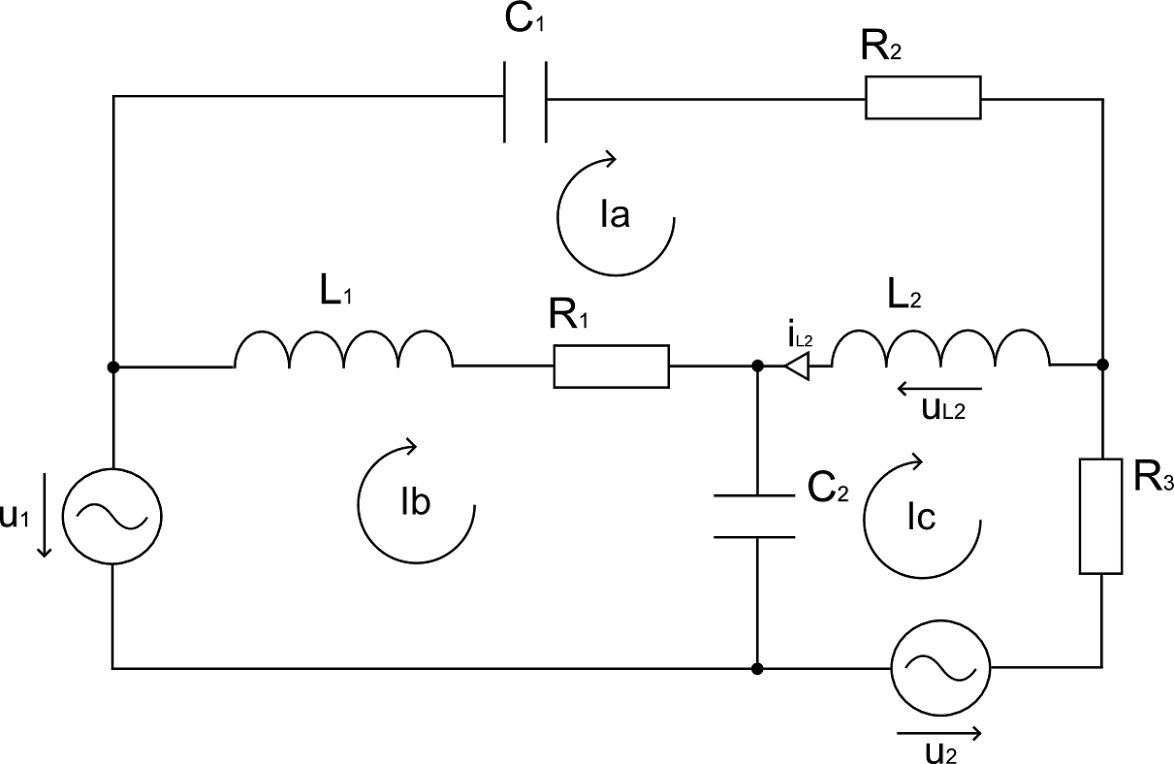
\includegraphics[height=6cm]{img/pr5}

1. Vypočítame uhlovú rýchlosť
\begin {equation*}
	\omega = 2\pi f = 2\pi * 95Hz = 596,9026 rad/s
\end {equation*}

2. Určíme si nasledujuce premenné
\begin{equation*}
    \begin{split}
	X_L = \omega L \\
	X_C = \frac{1}{\omega C}
   \end{split}
\end{equation*}

 3. Zostavíme  si rovnice
\begin{equation*}
    \begin{split}
	I_A &: -jX_{C_1}*I_A + R_1+I_A + jX_{L_2}*I_A - jX_{L_2}*I_C+ R_2*I_A - R_2 *I_B+jX_{L_1}*I_A-jX_{L_1}*I_B = 0 \\
	I_B &: jX_{L_1}*I_B - jX_{L_1}*I_A + R_2 *I_B - R_2*I_A - jX_{C_2}*I_B + jX_{C_2}*I_C - U_1 = 0 \\
	I_C &: -jX_{C_2}*I_C + jX_{C_2}*I_B + jX_{L_2} * I_C - jX_{L_2}*I_A + R_3 * I_C - U_2 = 0 \\
   \end{split}
\end{equation*}
\hrulefill
\begin{equation*}
    \begin{split}
	I_A*(R_1+R_2+jX_{L_2}+jX_{L_1}-jX_{C_1})-I_B*(R_2+jX_{L_1}) - I_C*jX_{L_2} = 0 \\
	-I_A*(R_2+jX_{L_1})+I_B*(R_2+jX_{L_1})-jX_{C_2}+I_C*jX_{C_2}=U_1 \\
	-I_A*jX_{L_2}+I_B*jX_{C_2}+I_C*(R_3+jX_{L_2}-jX_{C_2})=U_2
   \end{split}
\end{equation*}
4. Dosadíme hodnoty zo zadania do rovnice
\begin{equation*}
    \begin{split}
	I_A*(100+105+j44,7678+j95,5044-j10,8085)-I_B*(105+j95,5044) - I_C*j44,7678 = 0 \\
	-I_A*(105+j95,5044)+I_B*(105+j95,5044-j23,9331)+I_C*j23,9331=65 \\
	-I_A*j44,7677+I_B*j23,9331+I_C*(145+j44,7678-j23,9331)=60
   \end{split}
\end{equation*}
\hrulefill
\begin{equation*}
    \begin{split}
	I_A*(205+j129,4637)-I_B*(105+j95,5044) - I_C*j44,7677 = 0 \\
	-I_A*(105+j95,5044)+I_B*(105+j71,5713)+I_C*j23,933=65\\
	-I_A*j44,7677+I_B*j23,9331+I_C*(145+j20,8347)=60
   \end{split}
\end{equation*}
5. Zostavíme maticu
\begin{equation*}
M = \begin{bmatrix}
	205 +j129,4637 & -105-j95,5044 & -j44,7677 & 0  \\
	 -105 -j95,5044 & 105+j71,5713 &  j23,9331 & 65 \\
	-j44,7677 & j23,9331& 145+j20,8347 & 60 \\
     \end{bmatrix}
\end{equation*}
6. Vypočítame $I_A$ a $I_B$ pomocou determinantov
\begin{equation*}
\begin{split}
M_0 &= \begin{bmatrix}
	205 +j129,4637 & -105-j95,5044 & -j44,7677  \\
	 -105 -j95,5044 & 105+j71,5713 &  j23,9331\\
	-j44,7677 & j23,9331 & 145+j20,8347 \\
     \end{bmatrix} \\
M_1 &= \begin{bmatrix}
	0 & -105-j95,5044 & -j44,7677  \\
	65 & 105+j71,5713 &  j23,9331\\
	60 & j23,9331 & 145+j20,8347 \\
     \end{bmatrix} \\
M_3 &= \begin{bmatrix}
	205 +j129,4637 & -105-j95,5044 & 0 \\
	 -105 -j95,5044 & 105+j71,5713 &  65\\
	-j44,7677 & j23,9331 & 60 \\
     \end{bmatrix}
\end{split}
\end{equation*}
\begin{equation*}
    \begin{split}
	det(M_0) &= (205 +j129,4637)*(105+j71,5713)*(145+j20,8347) + \\
	&+ (-105-j95,5044)*( j23,9331)*(-j44,7677) + \\
	&+(-j44,7677)*(-105 -j95,5044 )*(j23,9331) - \\
	&-(-j44,7677)*( 105+j71,5713) * (-j44,7677) - \\
	&-(205 +j129,4637 ) * (j23,9331) * (j23,9331 ) - \\
	&-(-105-j95,5044)*(-105-j95,5044) * (145+j20,8347) = \\
	&= 1433312,11898 + 1419123,14901j \\
	det(M_1) &= (-105-95,5044j)*(23,933j)*60 + \\
	&+(-44,7677j*65*23,9331j) - \\
	&-(-44,7677j)*(105+71,5713j)*60 - \\
	&-(-105-95,5044j)*(65)*(145+20,8347j) = \\
	&=874828,03977 + 1173584,40750j \\
	det(M_3) &=(205+129,4637j)*(105+71,5713j)*60 + \\
	&+ (-105-95,5044j)*65*(-44,7677j)  - \\
	&-(-105-95,5044j)*(-105-95,5044j)*60 - \\
	&-(205+129,4637j)*23,9331j*65 = \\
	&=544804,40424 + 479223,8550j 
    \end{split}
\end{equation*}

\begin{equation*}
    \begin{split}
	I_A = \frac{det(M_1)}{det(M_0)} = \frac{874828,03977 + 1173584,40750j}{1433312,11898 + 1419123,14901j} = (0,7176 + 0,1083j) A \\
	I_C = \frac{det(M_3)}{det(M_0)} = \frac{544804,40424 + 479223,8550j}{1433312,11898 + 1419123,14901j} = (0,3591 - 0,0212j) A
    \end{split}
\end{equation*}
\newpage
7. Následne vypočítame $I_2$ a $U_{L_2}$
\begin{equation*}
\begin{split}
I_2 = I_A - I_C = (0,7176 + 0,1083j) -  (0,3591 - 0,0212j) =(0,3585 + 0,1295j) A \\
U_{L_2} = jX_{L_2} * I_2 =j44,7677 * (0,3585 + 0,1295j)= (-5,7974 + 16,0492i) V
\end{split}
\end{equation*}

8. Vypočítame  \textcolor{red}{$U_{L_2}$}
\begin{equation*}
|U_{L_2}| = \sqrt{{Re}^2 + {Im}^2} = \sqrt{-5,7974^2 + 16,0492^2} =17,0642V
\end{equation*}

9. Zistíme fázovy posun \textcolor{red}{$\varphi_{L_2}$}
\begin{equation*}
\varphi_{L_2} = \arctan \frac{Im}{Re} = -\frac{16,0492}{5,7974} = -70,1389^{\circ}
\end{equation*}

10. Prevedieme do spravneho kvadrantu
\begin{equation*}
\varphi_{L_2} =  -70,1389^{\circ} + 180^{\circ} = 109,8611^{\circ}
\end{equation*}

% % % % % % % % % %  6. Priklad % % % % % % % % % % % % % % % % % % % % % % % % 
\newpage
\begin{center}
\textbf{Priklad 6, Varianta D}
\end{center}
\bigskip
Zostavte diferenciálnu rovnicu popisujúcu chovanie obvodu na obŕazku, ďalej ju upravte dosadením hodnôt parametru. Vypočítajte analytickej riešenie
$\mu_C = f(t)$. Urobte kontrolu výpočtu dosadením do zostavenej diferencialnej rovnice.
\bigskip

Zadané hodnoty

\begin{tabular} {|  c | c | c |}
\hline
C [F] & R[$\Omega$] & $\mu_C(0)$ [V] \\ \hline
25 & 30 & 2\\ \hline
\end{tabular}
\bigskip

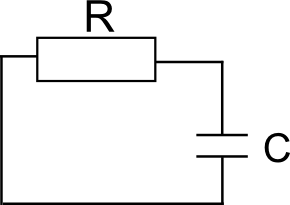
\includegraphics[height=5cm]{img/pr6}

1. Súčet napäti v smyčke je rovný 0
\begin {equation*}
	U_c + U_r = 0 \\	
\end{equation*}

2. Podľa Ohmovho zákona rozložíme $U_r$
\begin {equation*}
    \begin{split}
	U_r &= R * i \\
	U_c + R * i = 0 &=> i=-\frac{U_c}{R}
    \end{split}
\end{equation*}

3. Rozpíšeme axiom
 \begin {equation*}
    \begin{split}
	U'_c=\frac{1}{C}*(-\frac{U_c}{R}) \\
	R * C * U'_c = -U_c \\
	R * C * U'_c +  U_c = 0 \\
	u_c(0) = 5
    \end{split}
\end{equation*}

4.Zostavíme rovnicu
 \begin {equation*}
    \begin{split}
	750U'_c(t) + U_c(t) = 0 \\
	U_c(0) = 5 V \\
	750\lambda + 1 = 0 \\
	\lambda = -\frac{1}{750}
    \end{split}
\end{equation*}

5. Očakávany tvar:
 \begin {equation*}
    \begin{split}
	U_c(t) = c(t) * \epsilon^{\lambda t} \\
	U_c(t) = c(t) * \epsilon^{-\frac{1}{750}t}
    \end{split}
\end{equation*}
\newpage
6. Riešime rovnicu

a) Zderivujeme $U_c$

\begin {equation*}
	U'_c = c'(t) * \epsilon^{-\frac{1}{750}t} +c(t)  * \epsilon^{-\frac{1}{750}t} *(-\frac{1}{750}) \\
\end{equation*}

b) Dosadíme do pôvodnej rovnice

\begin{equation*}
	750 * (c'(t) * \epsilon^{-\frac{1}{750}t} + c(t) * \epsilon^{-\frac{1}{750}t} *(-\frac{1}{750}) = 0\\
\end{equation*}

c) Odpočítame členy
\begin{equation*}
	750 * (c'(t) * \epsilon^{-\frac{1}{750}t}) = 0
\end{equation*}

d) Súčin je rovný nule keď jeden z členov je nulový. Epsilon nebude nikdy rovné nule. Takže musi platiť $c'(t) = 0$. Derivácia je rovná nule keď derivujeme konštantu
\begin{equation*}
	\int c(t)\, \mathrm{d}t = 0 => c(t) = K
\end{equation*}

e) Dosadíme c(t) do očakávaneho tvaru
 \begin {equation*}
    \begin{split}
	U_c(t) = c(t) * \epsilon^{-\frac{1}{750}t} \\
	U_c(t) = K * \epsilon^{-\frac{1}{750}t}
    \end{split}
\end{equation*}

f) Dosadíme $U_c(0) = 5 V$
  \begin {equation*}
    \begin{split}
	5 = K * \epsilon^{-\frac{1}{750}*0} \\
	5 = K * 1 \\
	K = 5
    \end{split}
\end{equation*}

g) Výsledok:
\begin{equation*}
	U'_c(t) = 5 * \epsilon^{-\frac{1}{750}t}*(-\frac{1}{750})
\end{equation*}

7. Spravíme skúšku

a) Zderivujeme výsledne $U_c(t)$
\begin{equation*}
	U'_c(t) = 5* \epsilon^{-\frac{1}{750}t} *(-\frac{1}{750})
\end{equation*}

b) Dosadíme $U'_c(t)$ a $U_c(t)$ do pôvodnej rovnice
\begin{equation*}
    \begin{split}
	750 * U'_c(t) + U_c(t) = 0 \\
	750 * (5* \epsilon^{-\frac{1}{750}t} *(-\frac{1}{750})) + 5*\epsilon^{-\frac{1}{750}t} = 0 \\
	-5 * \epsilon^{-\frac{1}{750}t} + 5 * \epsilon^{-\frac{1}{750}t} = 0 \\
	0 = 0
    \end{split}
\end{equation*} 
% % % % % % % % % %  Suhrn vysledkov % % % % % % % % % % % % % % % % % % % % % % % % 
\newpage
\begin{center}
\textbf{Súhrn výsledkov}
\end{center}
\bigskip

    \begin{tabular}{|c|c|l|}
    \hline
    Príklad č.  & Varianta zadania & Výsledok                            \\ \hline
    1           & F                & $U_{R_7}$ = 29,59101V  \hspace{5mm} $I_{R_7}$ = 0,0896A \\ \hline
    2           & H                & $ U_{R_5}$ = 39,8449V \hspace{5mm}  $I_{R_5}$ = 0,1138A \\ \hline
    3           & D                & $U_{R_4}$ = 7967,8750V \hspace{2mm} $I_{R_4}$ = 21,5348A \\ \hline
    4           & F                & $|U_{C_1}|$ = 0,0646  \hspace{8mm} $\varphi_{C_1}$ = $128,8400^{\circ}$        \\ \hline
    5           & H                & $|U_{L_2}|$ = 17,0642  \hspace{7mm} $\varphi_{L_2}$ = $109,8611^{\circ}$         \\ \hline
    6           & D                & $U'_c(t) = 5 * \epsilon^{-\frac{1}{750}t} *(-\frac{1}{750})$                                  \\ \hline
    \end{tabular}



\end{document}